% Unofficial University of Cambridge Poster Template
% https://github.com/andiac/gemini-cam
% a fork of https://github.com/anishathalye/gemini
% also refer to https://github.com/k4rtik/uchicago-poster

\documentclass[final]{beamer}

% ====================
% Packages
% ====================

\usepackage[T1]{fontenc}
\usepackage{lmodern}
\usepackage[size=custom,width=91.44,height=60.96,scale=1.0]{beamerposter}
\usepackage{tikz}
\usetikzlibrary{arrows, positioning, calc} 
\usetheme{gemini}
\usecolortheme{cam}
\usepackage{graphicx}
\usepackage{booktabs}
\usepackage[numbers]{natbib}
\usepackage{pgfplots}
\pgfplotsset{compat=1.14}
\usepackage{anyfontsize}
\usepackage{simplebnf}
\usepackage{stmaryrd}
\usepackage{subcaption}
\usepackage{amsmath}
\usepackage{amssymb}
\usepackage{mathtools} 
\usepackage{tabularx} 
\usepackage{xcolor}
\usepackage[normalem]{ulem}


% ====================
% Lengths and Commands
% ====================

% If you have N columns, choose \sepwidth and \colwidth such that
% (N+1)*\sepwidth + N*\colwidth = \paperwidth
\newlength{\sepwidth}
\newlength{\colwidth}
\setlength{\sepwidth}{0.025\paperwidth}
\setlength{\colwidth}{0.3\paperwidth}

\newcommand{\separatorcolumn}{\begin{column}{\sepwidth}\end{column}}

\newlength{\redwidth}
\setlength{\redwidth}{\colwidth}

\newcommand{\redstep}[2]{%
  \noindent
  \makebox[\redwidth][c]{%
    \parbox[b]{0.5\redwidth}{\raggedleft\texttt{#1}}%
    \hfill
    \parbox[b]{0.10\redwidth}{\centering$\longrightarrow$}%
    \hfill
    \parbox[b]{0.5\redwidth}{\raggedright\texttt{#2}}%
  }%
}
% ====================
% Title
% ====================

\title{A Formal Model and Interactive Visualization of miniKanren Search Semantics}

\author{Brysen Pfingsten \and Jason Hemann}

%\institute[shortinst]{Seton Hall Univeristy}

% ====================
% Footer (optional)
% ====================

\footercontent{
  \href{https://minikanrenredex-prod.shu.edu}{minikanrenredex-prod.shu.edu} \hfill
  Petersheim 2025, South Orange, New Jersey \hfill
  \href{mailto:pfingsbr@shu.edu}{pfingsbr@shu.edu} \quad
  \href{mailto:hemannja@shu.edu}{hemannja@shu.edu}
}


% ====================
% Logo
% ====================

\logoleft{
  \includegraphics[height=6cm]{logos/logo3.pdf}
}



% ====================
% Body
% ====================

\begin{document}

% Refer to https://github.com/k4rtik/uchicago-poster
\addtobeamertemplate{headline}{}


\begin{frame}[t]
\begin{columns}[t]
\separatorcolumn


% ====================
% Abstract and Grammar
% ====================
\begin{column}{\colwidth}

% ====================
% Abstract
% ====================

  \begin{block}{Abstract}

Mechanized executable semantics are a valuable tool for implementers and users alike to better understand their programs' behavior. 
The need is particulary acute in the context of novel logic programming languages with complex search strategies. 
Few such tools exist for logic-based programming languages however, and existing work only models languages' search behavior at a somewhat coarse-grained level.
\textbf{In this work, we present the first small-step semantics for a logic language that models interleaving search at the level of individual goal execution.}
 The model is implemented in PLT Redex and allows users to step through the language's execution at a sub-interleave level.

\textbf{We also present a visualization tool implemented through interactive JS in the browser with our miniKanren Redex model at its core.}
This visualizer allows users to input their own miniKanren programs as Racket source code; these programs are transpiled to the language of our model. 
At each step, users can easily see the evaluation context of their programs, trace goals both to and from the source code and the search tree visualization, and readily understand the history of the computation that led parts of the current state to arise. 
This not only enables better performance analysis and a unique, visual way of debugging but also allows novice miniKanren programmers to more readily understand the semantics and structure underlying the miniKanren search evolution.

  \end{block}
  
% ====================
% Grammar
% ====================
  
\begin{alertblock}{Grammar}
\centering
\begin{figure}[htbp]
\begin{bnf}
$p$ ::=
| \texttt{(prog $\Gamma$ $e$)} :
;;
$\Gamma$ ::=
| \texttt{(($r_!$ $d$ $g$) ...)} :
;;
$d$ ::=
| \texttt{($x_!$ ...)} :
;;
$s$ ::=
| \texttt{()} $\vert$ \texttt{($g$ $\sigma$)} $\vert$ \texttt{($s \rightarrow s$)} $\vert$ \texttt{($s \leftarrow s$)} 
| \texttt{(($\top$ $\sigma$) + $s$)} $\vert$ \texttt{($s$ $\times$ $g$)} 
| \texttt{(proceed (($r$ $t$ ...) $\sigma$)} 
| \texttt{(delay $s$)} 
;;
$g$ ::= 
| $\top$ $\vert$ \texttt{($t$ =?\text{ $t$})} $\vert$ \texttt{($r$ $t ...$)}
| \texttt{($g \vee g$)} $\vert$ \texttt{($g \wedge g$)} $\vert$ \texttt{($\exists$ $d$ $g$)}
;;
$c$ ::=
| \textbf{natural}
;;
$x$ ::=
| (variable-prefix x\text{$\colon$})
;;
$r$ ::=
| (variable-prefix r\text{$\colon$})
;;
$t$ ::=
| $c$ $\vert$ \textbf{boolean} $\vert$ \textbf{string} $\vert$ \textbf{symbol}
| $x$ $\vert$ \texttt{empty} $\vert$ \texttt{($t$ $\colon$\text{ $t$})}
;;
$\sigma$  ::=
| \texttt{(state $sub$ $c$)}
;;
$sub$ ::=
| \texttt{(($c$ $t$) ...)}
;;
\end{bnf}
\caption{Abridged grammar of our language.}
\label{fig:bnf-grammar}
\end{figure}
  
\end{alertblock}


\end{column}

\separatorcolumn
% ==================================
% Evaluation Contexts and Interleave
% ==================================

\begin{column}{\colwidth}

% ===================
% Evaluation Contexts
% ===================
\begin{block}{Evaluation Contexts}
\begin{center}
\vspace{-1cm}
\begin{figure}[htbp]
\begin{bnf}
$E\Gamma$ : Program ::= 
| \texttt{(prog $\Gamma$ hole)}
;;
$Ev$ : Answer Stream ::= 
| \texttt{hole} $\vert$ \texttt{(($\top$ $\sigma$) + $Ev$)}
;;
$Es$ : Search Tree ::= 
| \texttt{hole} $\vert$ \texttt{($Es \leftarrow s$)} $\vert$ \texttt{($s \rightarrow Es$)} $\vert$ \texttt{($Es \times g$)}
;;
$Ex$ : Composition ::= 
| \texttt{$E\Gamma$$\llbracket$$Ev$$\llbracket$$Es$$\llbracket$hole$\rrbracket$$\rrbracket$$\rrbracket$}
\end{bnf}
\caption{Evaluation contexts of our language.}
\label{fig:eval-contexts}
\end{figure}
\vspace{-1.5cm}
\end{center}
\end{block}
  
% ==========
% Interleave
% ==========
  \begin{block}{Interleaving}

At the core of miniKanren's search is the interleave, which ensures fair evaluation by delaying each relation call until it reaches the top of the tree evaluation context. To preserve the visual shape of the tree while enabling this behavior, we implement a \textit{railway model} with directed disjunctions.

%%% Flow Chart %%%
\centering
\begin{figure}[htbp]
\vspace{-1cm}
\begin{tikzpicture}[
  node distance=2cm and 10cm,
  imagebox/.style={inner sep=0, anchor=center},
  every node/.style={anchor=center}
]

% --- Row 1 ---
\node[imagebox] (img1) at (0, 0) {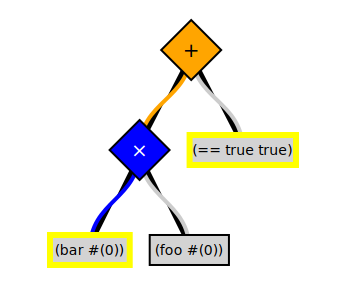
\includegraphics[height=8.7cm]{picts/int_1.pdf}};
\node[imagebox, right=of img1] (img2) {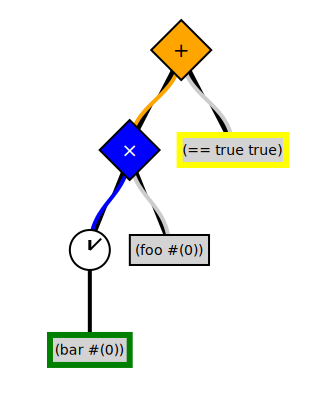
\includegraphics[height=8.7cm]{picts/int_2.pdf}};

% --- Row 2 ---
\node[imagebox, below=of img1] (img3) {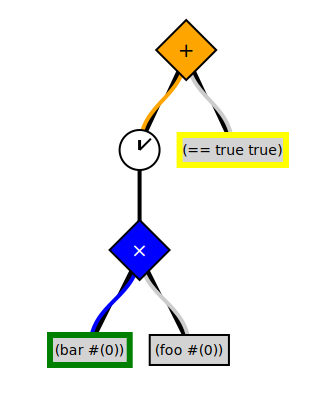
\includegraphics[height=8.7cm]{picts/int_3.pdf}};
\node[imagebox, right=of img3] (img4) {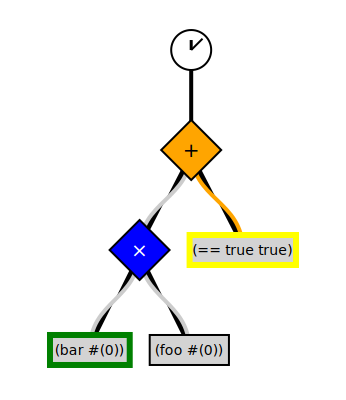
\includegraphics[height=8.7cm]{picts/int_4.pdf}};

% --- Row 3 ---
\node[imagebox, below=of img3] (img5) {\includegraphics[height=8.7cm]{picts/int_5.pdf}};
\node[imagebox, right=of img5] (img6) {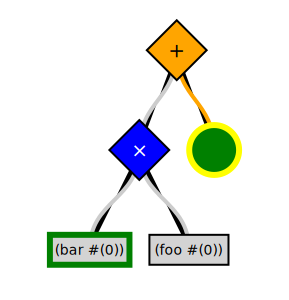
\includegraphics[height=8.7cm]{picts/int_6.pdf}};

% --- Horizontal arrows 
\draw[->, thick] (img1.east) -- (img2.west) node[midway, above] {\begin{tabular}{c}
																  \small Add Delay And \\
																  \small Mark As Proceed
																 \end{tabular}
																 };
\draw[->, thick] (img3.east) -- (img4.west) node[midway, above] {\begin{tabular}{c}
																	\small Propagate Delay Through \\
																	\small Disjunction And Point\\
																	\small Towards Right Side
																\end{tabular}
																	};
\draw[->, thick] (img5.east) -- (img6.west) node[midway, above] {\small Evaluate Right Side};

% --- Vertical arrows
\draw[->, thick] 
    ($(img2.south)+(0,-0.2)$) --  
    ++(0,-0.75) coordinate (down) -- 
    ($(down -| img3.north)$) coordinate (corner) -- 
    ($(img3.north)+(0,0.2)$)
    node[at=($(down)!0.5!(corner)$), above, yshift=2pt] { \begin{tabular}{c}
            \small Propagate Delay \\
            \small Through Conjunction
        \end{tabular}
        };

\draw[->, thick] 
    ($(img4.south)+(0,-0.2)$) --  
    ++(0,-0.75) coordinate (down) -- 
    ($(down -| img3.north)$) coordinate (corner) -- 
    ($(img5.north)+(0,0.2)$)
    node[at=($(down)!0.5!(corner)$), above, yshift=2pt] {\small Invoke Top Level Delay};

\end{tikzpicture}

\caption{Flow chart demonstrating interleave and railway behavior.}
\label{fig:flow_chart}
\end{figure}
  \end{block}

\end{column}

\separatorcolumn
% ================================
% Reduction Steps and Architecture
% ================================
\begin{column}{\colwidth}
% ===============
% Reduction Steps
% ===============
  \begin{exampleblock}{Select Reduction Steps}
  
% =====================================================
\heading{Distribute State Across Goals to Create Trees}
% =====================================================

\redstep
  {Ex$\llbracket$(($g_1$ $\vee$ $g_2$) $\sigma$)$\rrbracket$}
  {Ex$\llbracket$(($g_1$ $\sigma$) $\leftarrow$ ($g_2$ $\sigma$))$\rrbracket$}


\redstep
  {Ex$\llbracket$(($g_1$ $\wedge$ $g_2$) $\sigma$)$\rrbracket$}
  {Ex$\llbracket$(($g_1$ $\sigma$) $\times$ $g_2$)$\rrbracket$}

% =====================
\heading{Railway Model}
% =====================
We show here those reduction steps dealing with left-facing disjunctions and omit those dealing with right-facing disjunctions.
\begin{center}
\vspace{-1cm}
\redstep
  {Ex$\llbracket$((delay $s_1$) $\leftarrow$ $s_2$)$\rrbracket$}
  {Ex$\llbracket$(delay ($s_1$ $\rightarrow$ $s_2$))$\rrbracket$}

\redstep
  {Ex$\llbracket$(($\top$ $\sigma$) $\leftarrow$ $s$)$\rrbracket$}
  {Ex$\llbracket$(($\top$ $\sigma$) + $s$)$\rrbracket$}
  
\redstep
  {Ex$\llbracket$(() $\leftarrow$ $s$)$\rrbracket$}
  {Ex$\llbracket s \rrbracket$}

\redstep
  {Ex$\llbracket$((($\top$ $\sigma$) $\leftarrow$ $s_1$) $\leftarrow$ $s_2$)$\rrbracket$}
  {Ex$\llbracket$(($\top$ $\sigma$) $\leftarrow$ ($s_1$ $\leftarrow$ $s_2$))$\rrbracket$}
  
\redstep
  {Ex$\llbracket$(($s_1$ $\rightarrow$ ($\top$ $\sigma$)) $\leftarrow$ $s_2$)$\rrbracket$}
  {Ex$\llbracket$(($s_1$ $\rightarrow$ $s_2$) $\rightarrow$ ($\top$ $\sigma$))$\rrbracket$}
\end{center}

% ===========================
\heading{Delays and Proceeds}
% ===========================
Relation calls are wrapped with a proceed tag and then a delay tag. 
Delays at the top level are released and the next time the delayed relation call is encountered it will be expanded.
\begin{center}
\vspace{-1cm}
\redstep
  {\parbox[t]{0.45\redwidth}{\raggedleft\texttt{$Ex$$\llbracket$(($r_1$ $t$ ...) $\sigma$)$\rrbracket$}}}
  {\parbox[t]{0.45\redwidth}{\raggedright\texttt{$Ex$$\llbracket$(delay (proceed (($r_1$ $t$ ...) $\sigma$)))$\rrbracket$}}}

\redstep
  {(prog $\Gamma$ $Ev$$\llbracket$(delay $s$)$\rrbracket$}
  {(prog $\Gamma$ $Ev$$\llbracket$$s$$\rrbracket$)} 
\end{center}
\end{exampleblock}

% ============
% Architecture
% ============

\begin{block}{Architecture}
Our visualizer is implemented as a web app using D3 to render our trees. 
Our API is responsible for fulfilling the requests of the user by either sending a cached state if it exists or stepping the program and sending back the corresponding JSON. 
\\ 
You can try it out now at \textcolor{blue}{minikanrenredex-prod.shu.edu}.

\begin{figure}[htbp]
	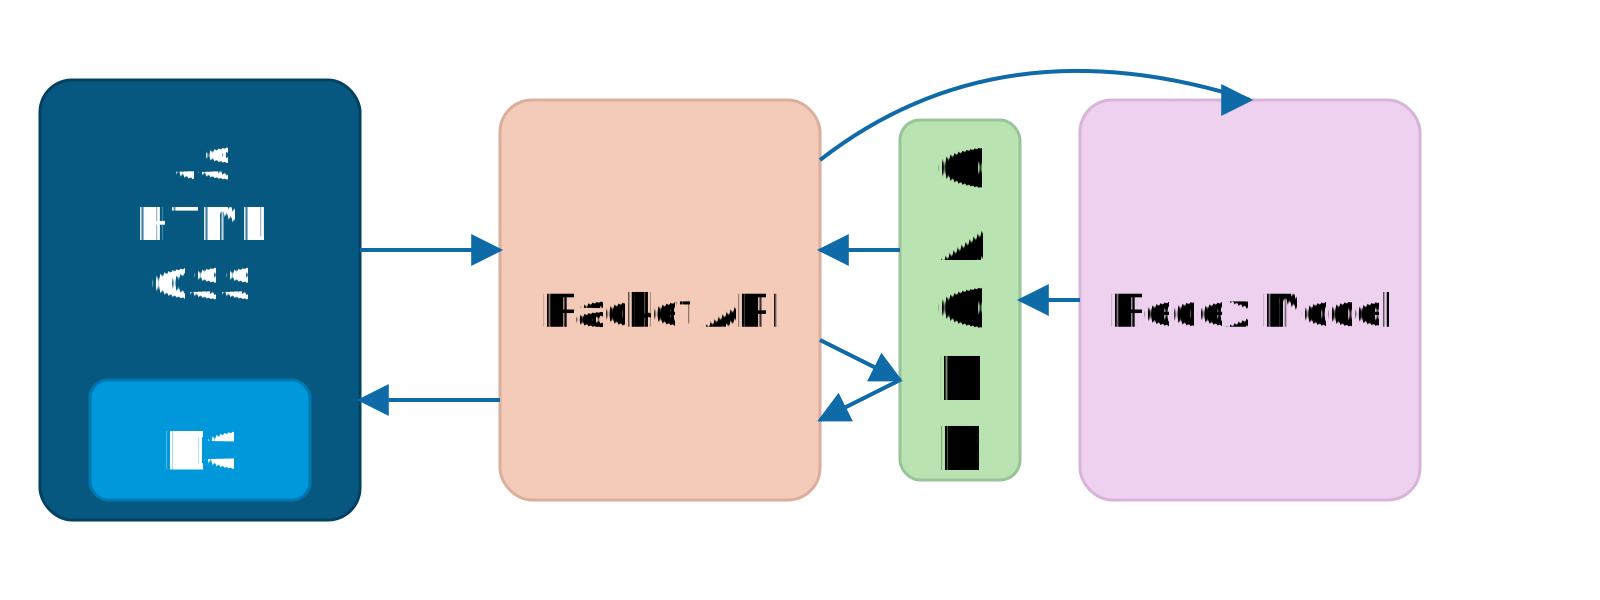
\includegraphics[height=7.8cm]{picts/architecture.pdf}
\caption{The architecture of our application.}
\label{fig:architecture}
\end{figure}

\end{block}

\end{column}

\separatorcolumn
\end{columns}
\end{frame}

\end{document}
